
En este apartado enumeraremos los objetivos que se pretenden alcanzar por parte de la alumna durante el desarrollo de este proyecto final de carrera.\par
Esto nos permitirá acotar el alcance del proyecto y establecer los hitos a alcanzar, permitiendo elaborar una planificación lo más precisa posible.\medskip\par

Los objetivos a lograr son los siguientes:
\begin{itemize}
	\item Demostrar la habilidad para emprender un proyecto parcialmente autónomo a partir de lo estudiado durante el periodo de formación académica en la Ingeniería Informática.
	\item Comprender la estructura de los informes médicos de tipo DICOM-SR y ser capaz de interpretar su contenido.
	\item Desarrollar una aplicación que realice el análisis sintáctico y semántico de ficheros DICOM-SR.
	\item Desarrollar una aplicación Android genérica para generar interfaces que permitan la introducción de informes DICOM-SR en base a plantillas.
	\item Desarrollar una aplicación que a partir de un fichero DICOM-SR genere los ficheros necesarios para completar la aplicación Android básica para el informe concreto de entrada. 
	\begin{itemize}
		\item Comprender la generación de código haciendo uso de plantillas.
	\end{itemize}
	\item Realizar las pruebas pertinentes a la aplicación para un informe concreto. Estas pruebas las aplicaremos exhaustivamente a 4 ontologías:
	\begin{itemize}
		\item Exploración de mama.
		\item Mamografía.
		\item Ultrasonidos
		\item Resonancia magnética.
	\end{itemize}
	Y consistirán en realizar las siguientes tareas:
	\begin{itemize}
		\item Generar el código XML para soportar la internacionalización
		\item Generar el código XML que desarrolle la interfaz de usuario. 
		\item Generar el código XML con las propiedades de la aplicación Android.
		\item Generar el código java que codifique los modelos de clase del informe. 
		\item Generar el código java que codifique las interacciones entre actividades.
		\item Integrar todo el código generado dentro de la aplicación base de Android. 
		\item Comprobar su correcto funcionamiento en terminales físicos.
	\end{itemize}
\end{itemize}
\medskip\par
Aunque no sea estrictamente necesario, hemos creado un diagrama de Gantt que podemos ver en la figura \ref{fig:gantt}, que nos ayude a planificar el tiempo para lograr los objetivos que acabamos de describir.\par
\begin{figure}[ht]
\centering
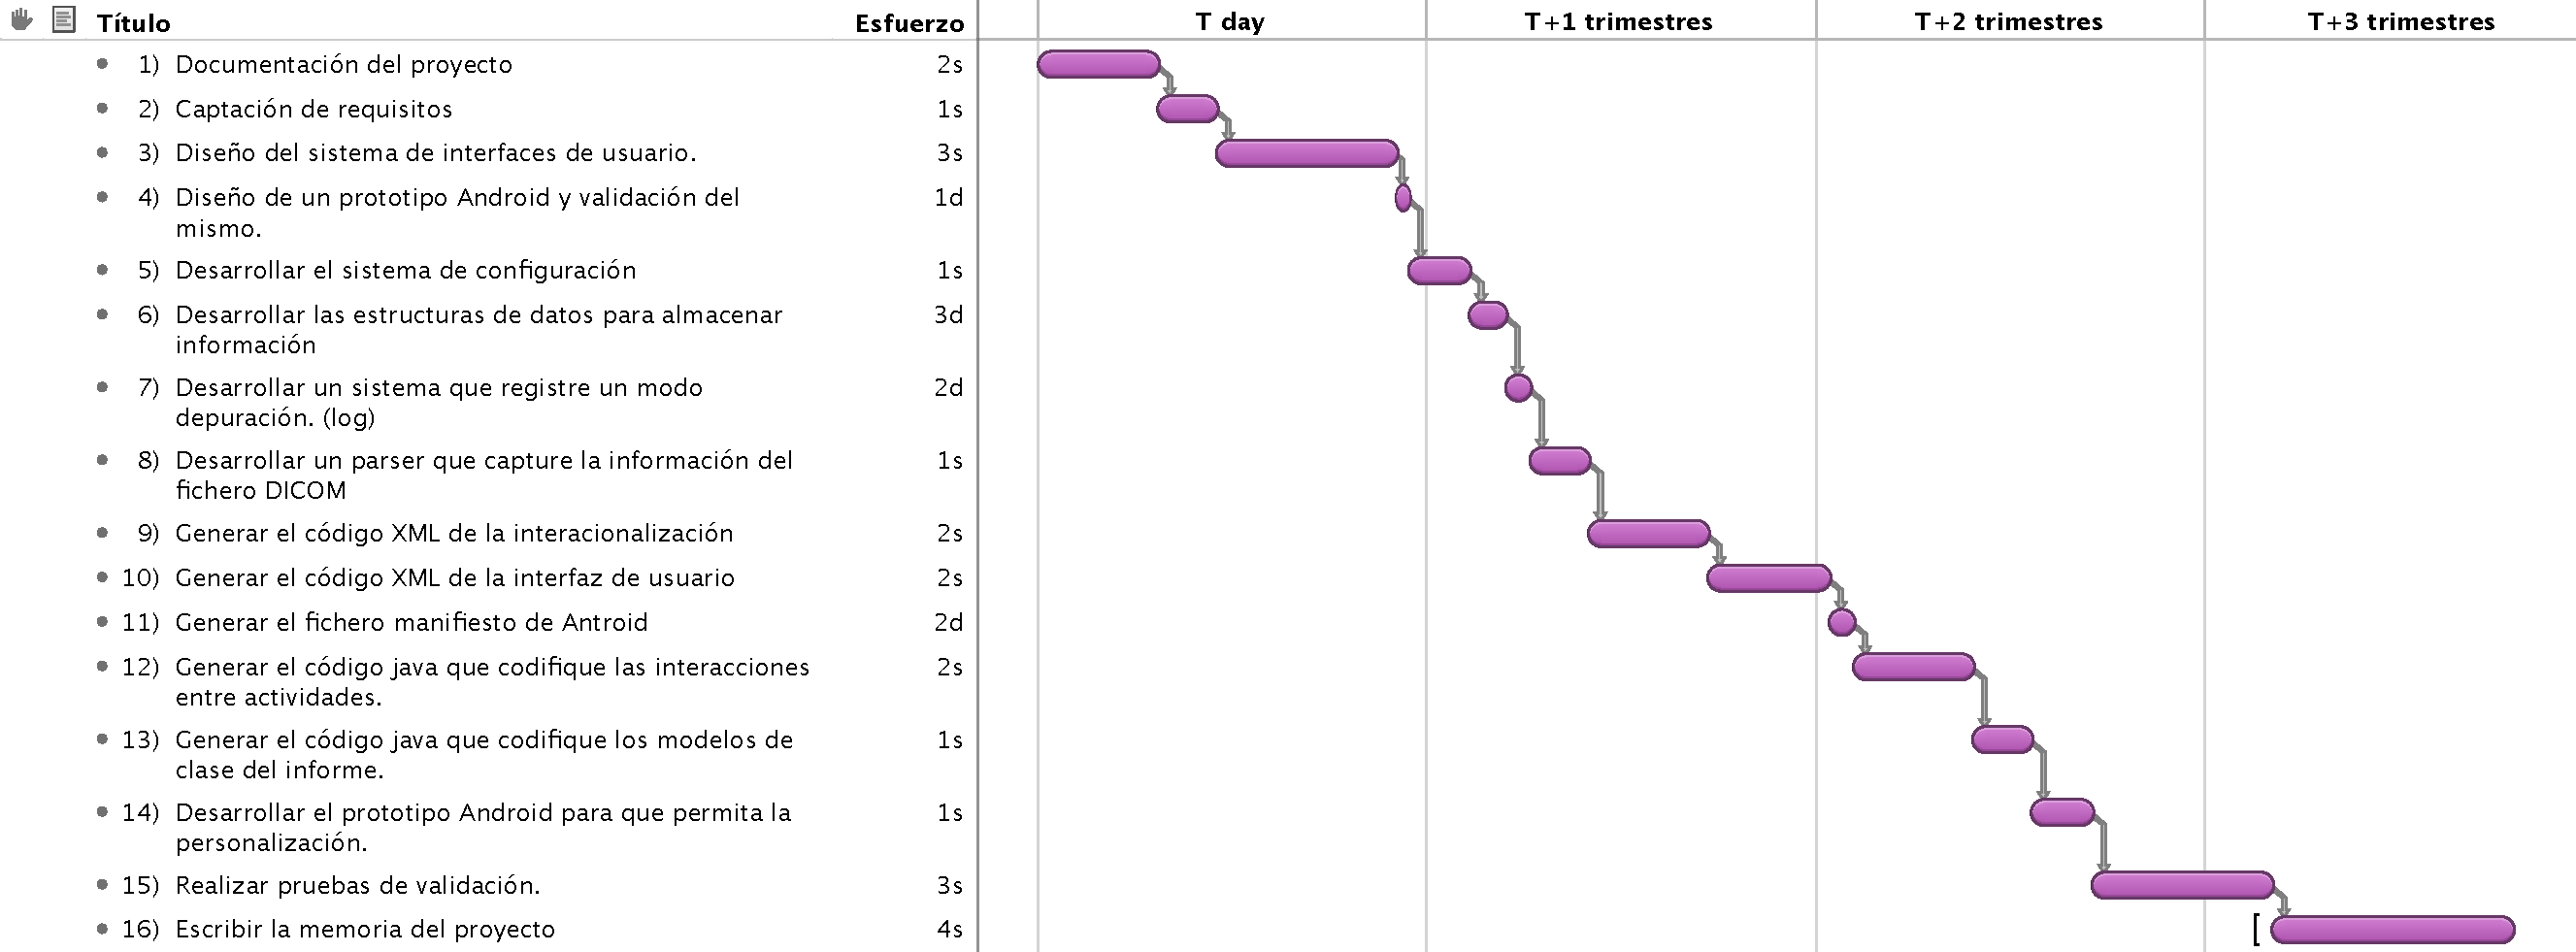
\includegraphics[scale=0.3]{./imgs/gantt.pdf}
\caption{Diagrama de Gantt}
\label{fig:gantt}
\end{figure}
